\subsection{Synchrotron X-ray source and ray tracing}
The synchrotron X-ray source and propagation from the source to the target is
realized with the \href{http://ftp.esrf.eu/pub/scisoft/Oasys/readme.html}{Oasys}
software package developed by Luca Rebuffi and Manuel Sanchez del Rio
 using the x--ray tracing
capability via the code \textit{Shadow3}. Installation scripts and the wiki page for Oasys 1.0 can be
found at
\href{https://github.com/srio/oasys-installation-scripts/wiki}{https://github.com/srio/oasys-installation-scripts/wiki}.
\href{https://github.com/srio/ShadowOui-Tutorial}{Tutorials for
Oasys and ShadowOUI} cover the various steps in preparing, executing, and
analysing the raytracing simulation. As part of preparation for the new High Power
Laser Facility (HPLF), that will be installed on the ID24 beamline at the ESRF,
the current energy dispersive X-ray absorption beamline has been simulated using
Oasys.
The ID24 beamline workflow for Oasys can be obtained from the EUCALL Data
Repository at Zenodo \cite{Briggs2017.zenodo.886451}.

\subsection{Particle matter interaction: long pulse laser}
The long pulse laser interaction with sample is performed using the Esther hydrocode. 
Here we have demonstrated a `simple' experiment, that could be performed on the 
ID24 XAS beamline, where a 6 ns flat top laser pulse (1064 nm) sends an ablative 
driven shockwave through a 45 um CH-plastic ablator and into a 5 um Fe layer. A 
tutorial that describes how the input files are generated (and how output data is 
obtained) is provided on the Simex wiki page \textbf{(NOTE: LATEX DOESN'T LIKE 
THE UNDERSCORE CHARACTER IN THE LINK TO WIKKI PAGE)}; all example input 
and output files are available from the EUCALL Data Repository at Zenodo
 [https://doi.org/10.5281/zenodo.883106]. The pressure in the Fe sample at t = 8.9 ns 
 (laser pulse begins at t = 0 ns) is shown in figure \ref{fig:hydro}. 
 
 The pressure, temperature, density and velocity can all be obtained at a given 
 time step from the output files that Simex converts to opmd format. Upon 
 completion of the code, it is then possible to adjust laser parameters to reach 
 different pressure-temperature conditions in the Fe sample. The P-T condition 
 where the pressure is uniform through the whole of the sample is then stored and 
 XAS modelling can be performed to simulate the expected EXAFS signal at 
 the compressed state.

\begin{figure}
  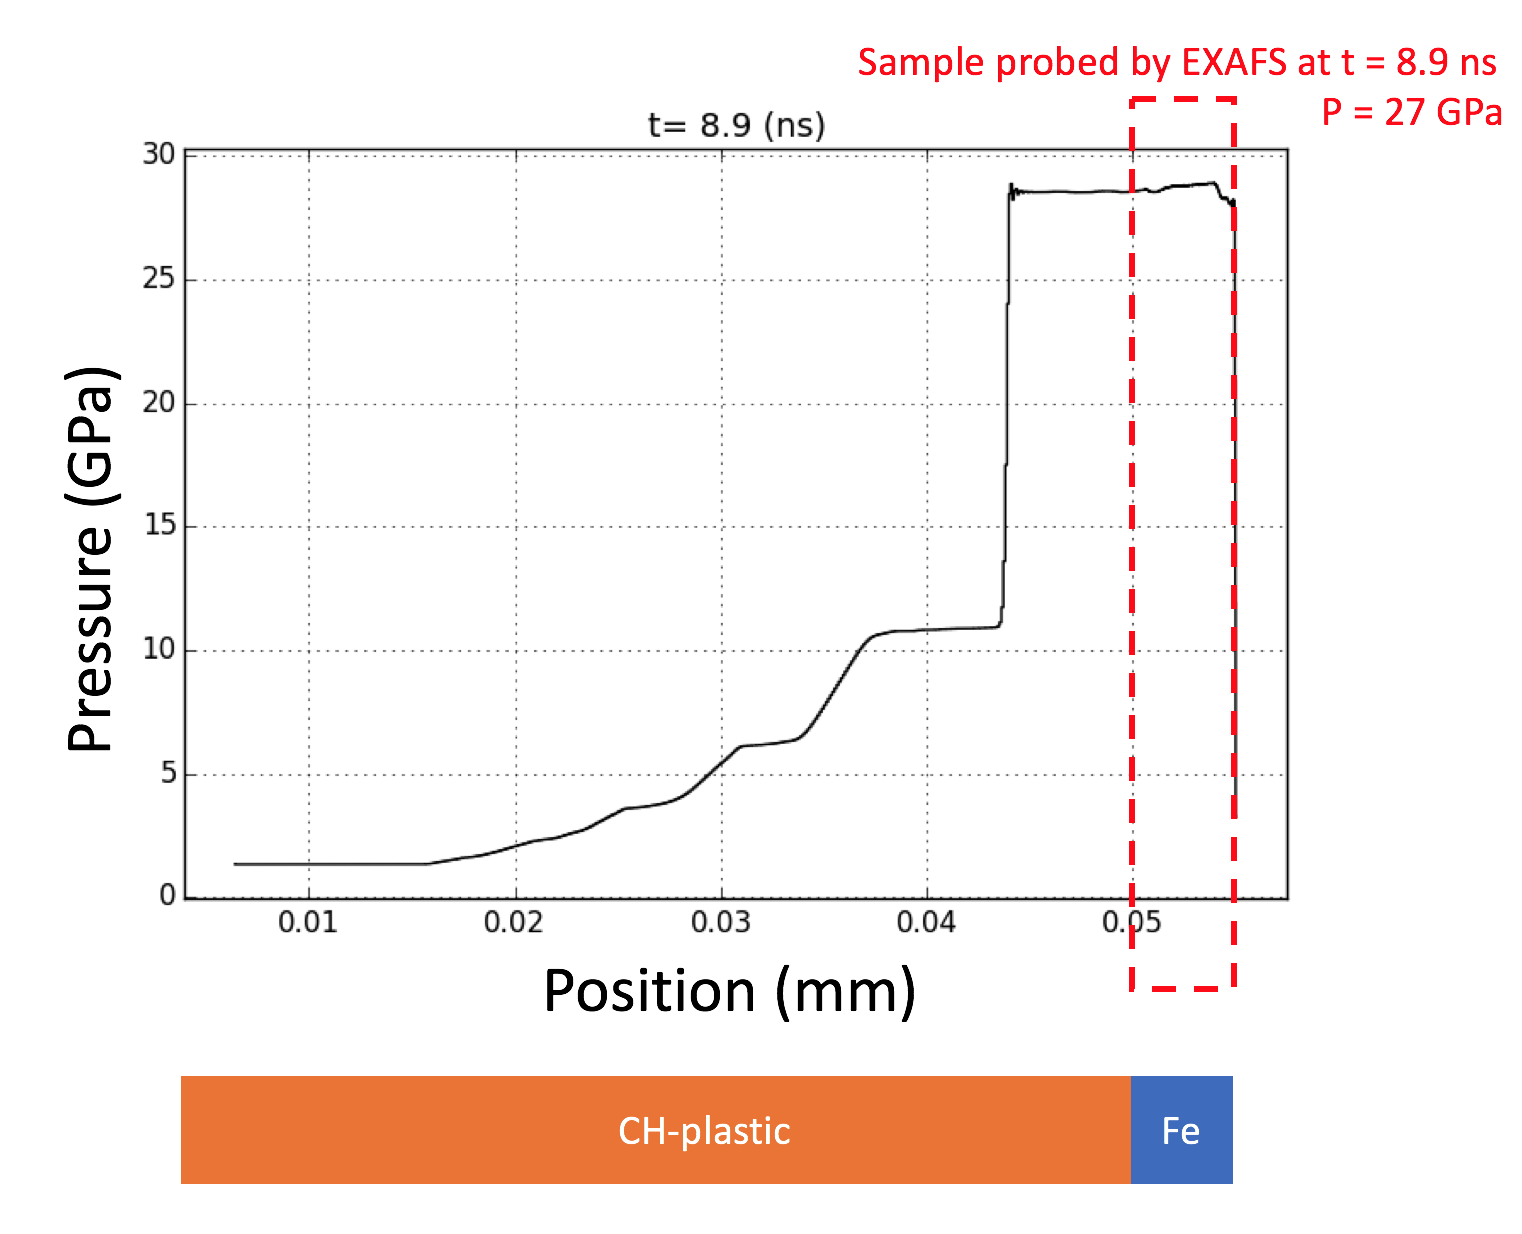
\includegraphics[width=4.822in]{figures/SIMEX-Fe-Shock.png}
  \caption{%
    Something here%
  }
  \label{fig:hydro}
\end{figure}

\subsection{Modelling of EXAFS}
In this simple example, to show the interoperability with the hydrocode,
we run through the requirements that are necessary for
simulation (fitting) of EXAFS data relevant to a sample experiment obtain signal
from a \SI{5}{\micro\metre} thick Fe foil. The simulation will be carried out for
ambient conditions Fe foil; a future enhancement of SIMEX will take P-T
conditions from hydrocode simulations before performing high-pressure
XANES/EXAFS calculations.

To validate the EXAFS simulations, we compare the simulated spectrum with raw
data obtained from an X-ray absorption beamline at the ESRF synchrotron. The
normalized XAS spectrum for a \SI{5}{\micro\metre} thick Fe foil is shown in figure 1.
\begin{figure}
  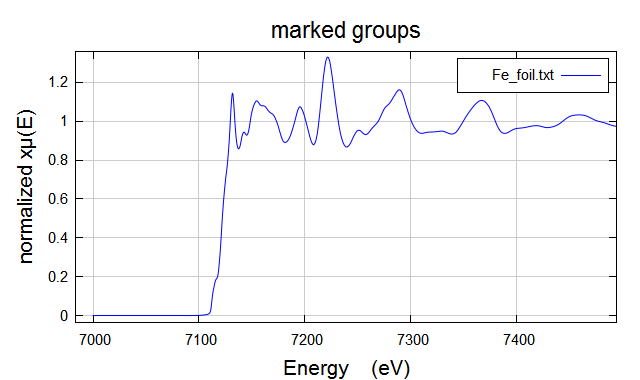
\includegraphics[width=4.822in,height=2.528in]{figures/Task42210-img001.png}
  \caption{%
    X-ray absorption spectra collected at BM23 (EXAFS beamline, ESRF) of
    a \SI{5}{\micro\metre} thick iron foil.%
  }
  \label{fig:xafs_fig1}
\end{figure}
Calculations of XAFS spectra are performed using the FEFF package. FEFF uses a
single input file to select which modules should be run inside the program and
what parameters should be used. The material of interest is contained within
this input file based on its crystallographic parameters and atomic positions.
The ATHENA program is able to combine crystallographic input files (.cif format)
for a chosen material into the FEFF .inp format. The .cif files can typically be
found from most crystallographic database websites or can be manually created
using gui programs such as VESTA. FEFF is then run to calculate the paths
between atoms and is then saved / exported for use by other third party programs
(such as ARTEMIS) to compare with actual data.

\subsubsection{Artemis User Guide} A more comprehensive user guide for running ARTEMIS
/ FEFF can be found at
\href{http://bruceravel.github.io/demeter/artug/index.html}{http://bruceravel.github.io/demeter/artug/index.html}.

\begin{figure}
  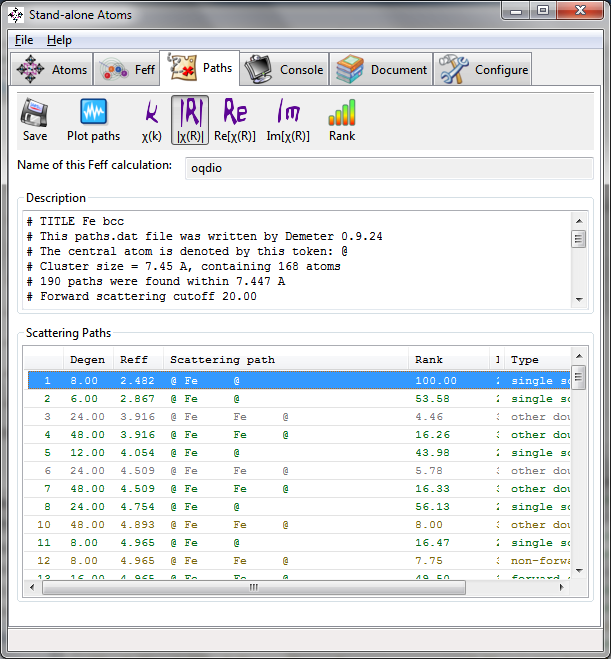
\includegraphics[width=4.3063in,height=4.6465in]{figures/Task42210-img002.png}
  \caption{%
    Screenshot of the output data collected in the ATOMS software after
    running Feff simulation of Fe at ambient conditions.
  }
  \label{fig:xafs_fig2}
\end{figure}

\begin{figure}
  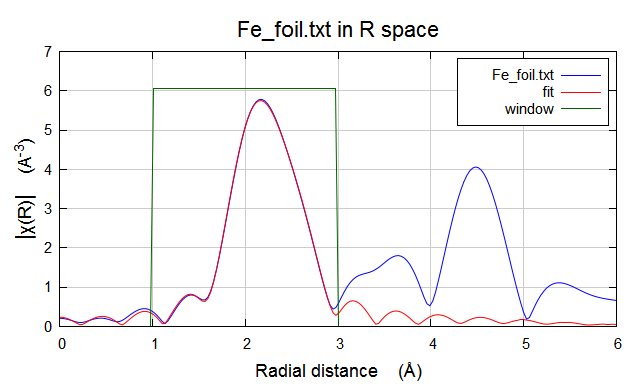
\includegraphics[width=4.852in,height=2.9173in]{figures/Task42210-img003.png}
  \caption{%
    Fitting of the first Fe shell from FEFF calculations (red) to Fe EXAFS
    data collected on BM23 beamline, ESRF (blue)
  }
  \label{fig:xafs_fig3}
\end{figure}

\subsubsection{Simulating XANES at shock conditions}
Shock compression experiments on Fe have previously been carried out at the ESRF
\cite{Torchio2016}. In that study,
simulations of the XANES at shock conditions were carried out using the ABINIT
code and are shown below in figure 4.

\begin{figure}
  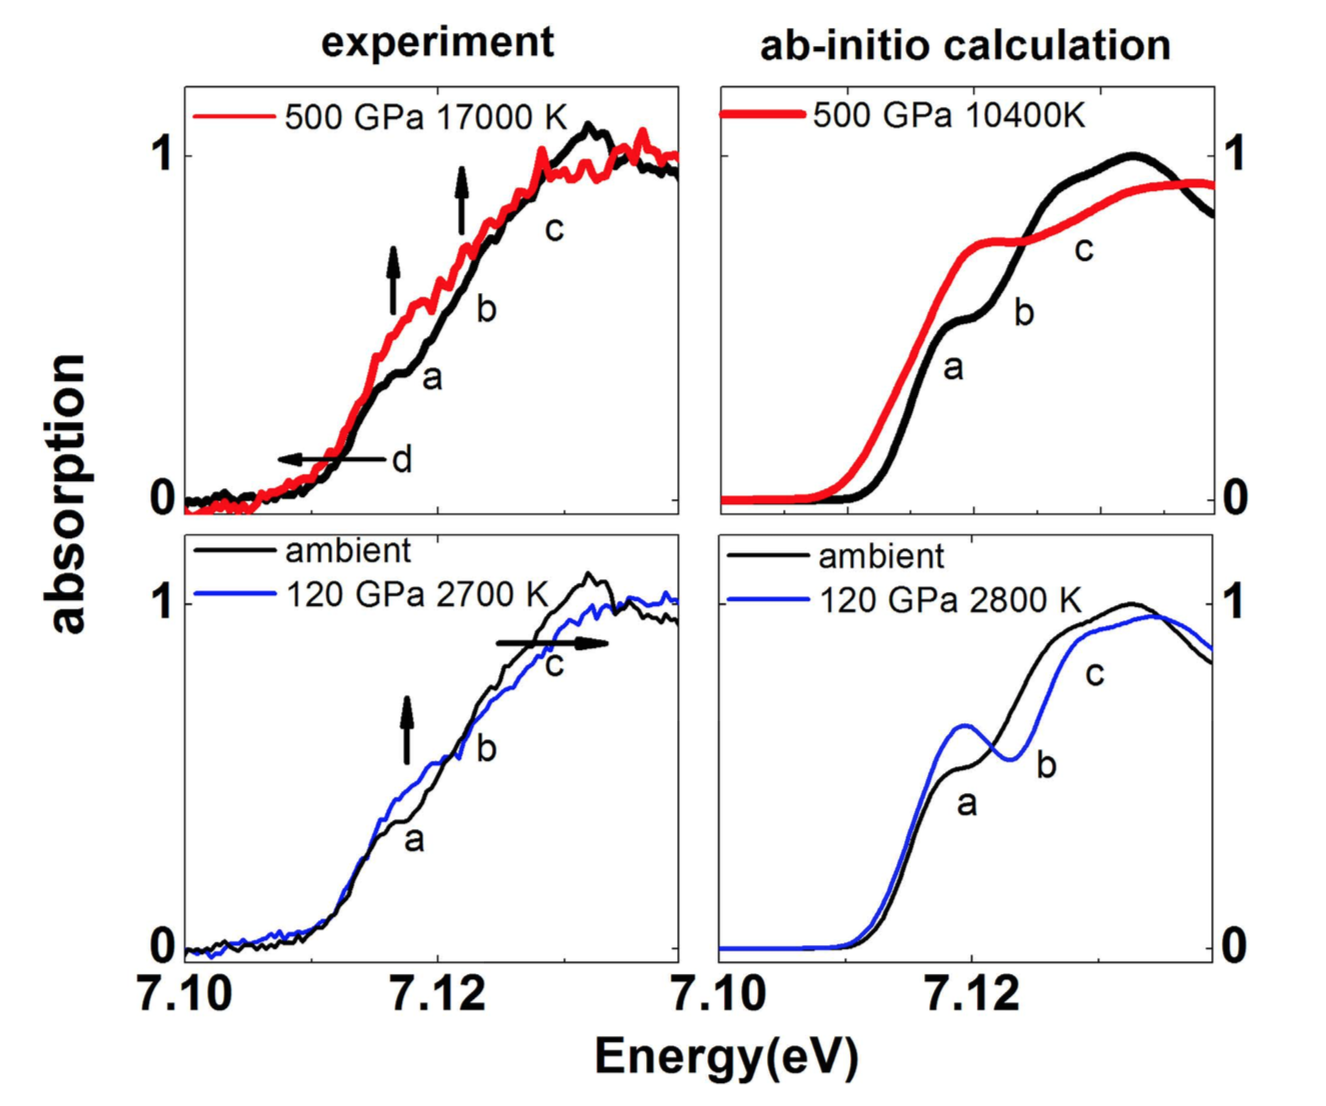
\includegraphics[width=4.3063in,height=3.5945in]{figures/Task42210-img004.png}
  \caption{%
    Comparisons of the absorption edge of Fe between experiments (left
    panels) and ab-initio calculations (right panels) at
    \SIlist{120;150}{\giga\pascal}. Figure
  taken from Ref.~\cite{Torchio2016}.
  }
  \label{fig:xafs_fig4}
\end{figure}
